\documentclass[11pt]{article}

\usepackage[utf8]{inputenc} % Required for inputting international characters
\usepackage[T1]{fontenc} % Output font encoding for international characters

\usepackage{mathpazo} % Palatino font
\usepackage{graphicx}
\usepackage{geometry}
\usepackage{float}
\usepackage{amsmath}
\usepackage{tabu}
\usepackage{array}
\usepackage{cellspace}
\usepackage[table]{xcolor}
\usepackage{multirow}
\usepackage{multicol}
\usepackage{parskip}

\usepackage{titlesec}
\titlespacing\subsection{0pt}{1pt plus 4 pt minus 2pt}{1pt plus 4 pt minus 2pt}

\renewcommand{\baselinestretch}{1.25}
\geometry{margin=0.75 in}

\begin{document}

%----------------------------------------------------------------------------------------
%	TITLE PAGE
%----------------------------------------------------------------------------------------

\begin{titlepage} % Suppresses displaying the page number on the title page and the subsequent page counts as page 1
	\newcommand{\HRule}{\rule{\linewidth}{0.5mm}} % Defines a new command for horizontal lines, change thickness here
	
	\center % Centre everything on the page
	
	%------------------------------------------------
	%	Headings
	%------------------------------------------------
	
	\textsc{\LARGE Portland State University
}\\[.25cm] % Main heading such as the name of your university/college
	
	\textsc{\Large Department of Electrical and Computer Engineering }\\[.5cm] % Major heading such as course name

\includegraphics[width=0.2\textwidth]{images/psuLOGO}\\[.5cm]
	\textsc{\LARGE ECE 411 - Industry Design Process }\\[0.75cm] % Minor heading such as course title
	
		\textsc{\Large Professor Andrew Greenberg, MS\\
Professor of Electrical \& Computer Engineering
 }\\[.75cm]
	
	%------------------------------------------------
	%	Title
	%------------------------------------------------
	
	\HRule\\[0.4cm]
	
	{\huge\bfseries Project Design Specification}\\[0.4cm] % Title of your document
	
	\HRule\\[1.5cm]
	
	%------------------------------------------------
	%	Author(s)
	%------------------------------------------------
	
%	\begin{minipage}{0.4\textwidth}
%		\begin{flushleft}
%			\large
%			\textit{By:}\\
%		 \textsc{Kimball S. Davis} % Your name
%		\end{flushleft}
%	\end{minipage}
%	~
%	\begin{minipage}{0.4\textwidth}
%		\begin{flushright}
%			\large
%			\textit{Professor of Electrical \& Computer Engineering}\\
%		 \textsc{Professor Branimir Pejcinovic, Ph.D.} % Supervisor's name
%		\end{flushright}
%	\end{minipage}
	
	% If you don't want a supervisor, uncomment the two lines below and comment the code above
	\Large{Group \#16:}\\
		 \Large\textsc{Kimball S. Davis, Jason Houlihan, \& Nathan Lutterman} % Your name
	
	%------------------------------------------------
	%	Date
	%------------------------------------------------
	
	\vfill\vfill\vfill\vfill % Position the date 3/4 down the remaining page
	
	{\large\today} % Date, change the \today to a set date if you want to be precise
	
	%------------------------------------------------
	%	Logo
	%------------------------------------------------
	
	%\vfill\vfill
	%\includegraphics[width=0.2\textwidth]{PSULOGO}\\[1cm] % Include a department/university logo - this will require the graphicx package
	 
	%----------------------------------------------------------------------------------------
	
	\vfill % Push the date up 1/4 of the remaining page
	
\end{titlepage}

%----------------------------------------------------------------------------------------
\setlength{\columnsep}{.2 in}

\setlength{\parskip}{0pt}

	
\section*{Executive Summary}
Everyday medical, industrial, and home applications need a precise temperature controller. Our digital temperature controller is primarily used to control the temperature of any device whose temperature keeps fluctuating and requires a constant watch. This system can be used in any organization where it is very important to maintain specific temperatures. This system is better than analogue/ thermostat systems, which have poor accuracy. Its main use is for temperature control of an incubator where maintaining a precise temperature is very important.\\

The digital temperature controller provides the temperature information on a LCD display, and when the temperature exceeds the set point, the load (heater) switches off. For the purpose of our practicum project, a lamp will be used as a load for demonstration purpose. If time permits we would also add a fan to cool the device when the temperature exceeds the set limit. Therefore the system keep switching the lamp, and fan, on and off which automatically controls the temperature of the system.\\

The digital temperature controller uses a microcontroller from the 8051 family (AT89S52), which is the bulk of the application. The display unit consists of four seven segment display pins which are interfaced to the microcontroller. The digital temperature sensor (DS1621) is interfaced to the microcontroller for sensing the temperature conditions. The system also provides four push buttons switches for adjusting, and setting the temperature. The microcontroller then polls the temperature information through a digital temperature sensor and displays the seven segment display units. When the corresponding temperature exceeds the set point, the lamp/fan automatically switches off/on.\\

The following are some examples of digital temperature controller using a microcontroller:
\begin{itemize}
    \item Outdoor use involving potential chemical contamination or electrical interference.
    \item Outdoor use involving potential chemical contamination or electrical interference.
    \item Medical equipment, amusement machines, vehicles, safety equipment, and installations subject to separate industry or government regulations.
    \item Systems, machines, and equipment that could present a risk to life or property.
    \item HVAC control for industrial and residential applications.
\end{itemize}

\pagebreak

\section*{Brief Market Analysis} 

While there are many uses for precision programmable temperature control units, home heating and cooling is a place where there is an available market, and a need for better more efficient thermostats. In a survey from the U.S. Energy Information Agency (EIA) it was found that while over 87$\%$of homes were equipped with HVAC, only roughly 52$\%$ of them had programmable thermostats. There is plenty of competition in the market from industry giants such as General Electric, Honeywell, and Emerson who currently have many similar products available some even offering entire smart home systems.\\

Where there is room for growth in the market is in ease of use, customization, and peripherals. A few things that would make our product stand out from the rest would be: LCD touchscreens, data logging for predictive thermostat control,and RFID implementation for personalized thermostat settings from room to room.\\

Ideally there would be several models with the same basic TCU as the engine. The price would depend on if it was the base model or the more advanced models with more functions/peripherals. Similar products on the market range from \$60 to \$100 for a basic programmable thermostat, and up to \$250 for the more advanced programmable models.


\section*{Requirements}
\subsection*{Must}
\begin{itemize}
    \item Accurately detect temperature 
    \item Accurately report temperature through a display
    \item Have a programmable temperature setting
    \item Switch between heating and cooling modes when temperature threshold is exceeded 
    \item Be easy to use
    \item Use an AT89S52 microcontroller
    \item Use > 25\% SMT components
    \item Have the processor on the PCB 
    \item Have in circuit Programming capabilities
    \item Use a two or more layer PCB, with solder mask and at least a top-side silk screen
    \item Area between 9-900 $cm^2$, and a linear dimension between 2-30 cm

\end{itemize}

\subsection*{Should}

\begin{itemize}

    \item Be as small as possible
    \item Have an enclosure

\end{itemize}
		
\subsection*{May}

\begin{itemize}

    \item Have data logging capabilities
    \item Have an LCD screen
    \item Include RFID programming

\end{itemize}

\section*{System Architecture}
The level 1 block diagram for our proposed design can be seen below.
	
	\begin{figure}[H]
	\centering
	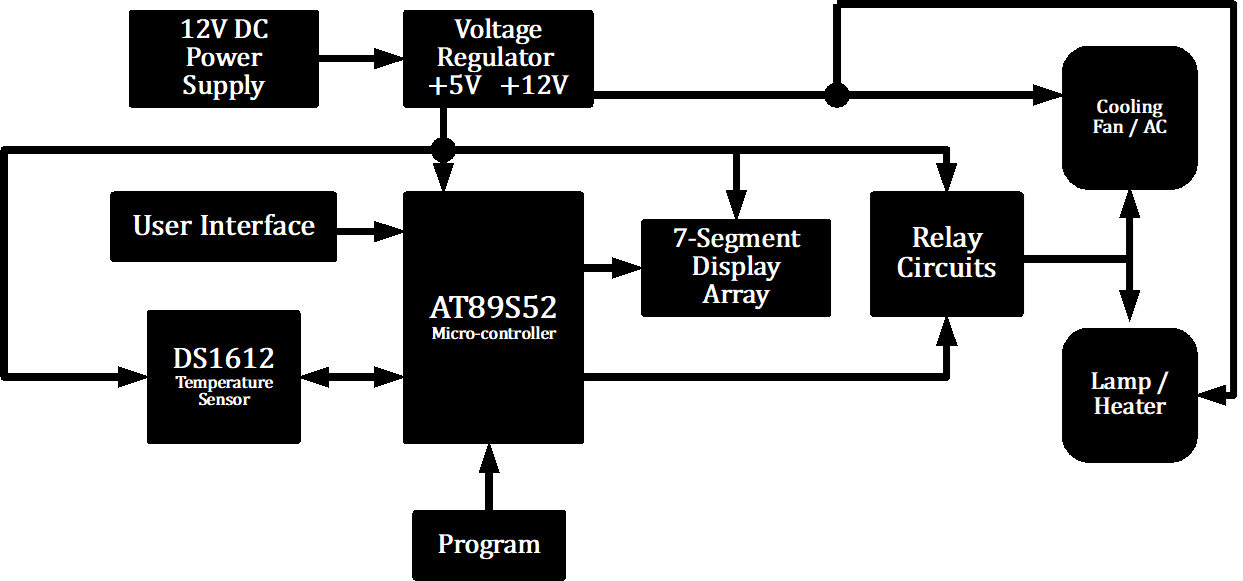
\includegraphics[width=5in]{images/TCU}
		\caption{\textit{Block diagram of digital temperature controller.}}
	\end{figure}

\section*{Design Specifications}

\subsection*{Sensors}
\begin{itemize}
	\setlength\itemsep{-2px}
    \item Digital Temperature Sensor(DS1621)
    \item Push Buttons.

\end{itemize}

\subsection*{Actuators}
\begin{itemize}
	\setlength\itemsep{-2px}
    \item 7 Segment display pins
    \item Lamp and fan
    \item LEDs
\end{itemize}

\subsection*{Controller}
\begin{itemize}
	\setlength\itemsep{-2px}
    \item Microcontroller (AT89S52)
\end{itemize}

\subsection*{Additional}
\begin{itemize}
	\setlength\itemsep{-2px}
    \item Voltage regulator (LM7805C)
    \item Transistors (2N2222) 
    \item 5V Relays (JQC-3F)
    \item Resistors/Capacitors

\end{itemize}
	
\end{document}

